%+++++++++++++++++++++++++++++++++++++++++++++++++++++++++++++++++++++++++++++++
%+++++++++++++++++++++++++++++++++++++++++++++++++++++++++++++++++++++++++++++++
%everything belong to gui: 3D visualization, mouse, keys, ...
%
\mysectionlabel{Graphics and visualization}{sec:graphicsVisualization}
%
The 3D OpenGL graphics renderer window is kept simple, but useful to see the animated results of the multibody system.
The graphics output is restricted to a 3D window (renderwindow) into which the renderer draws the visualization state of the \texttt{MainSystem} \texttt{mbs}.
Note that visualization parameters can be widely changed (more than 200 parameters ...), see \refSection{sec:overview:basics:visualizationsettings}.


%+++++++++++++++++++++++++++++++++++++++++++++++++++++++
%+++++++++++++++++++++++++++++++++++++++++++++++++++++++
\mysubsectionlabel{Mouse input}{sec:GUI:sec:mouseInput}
The following table includes the mouse functions:
%
\startGenericTable{| p{4cm} | p{4cm} | p{8cm} |}
\rowTableThree{\mybold{Button}}{action}{\mybold{remarks}}
\rowTableThree{\mybold{left mouse button}}{move model }{keep left mouse button pressed to move the model in the current x/y plane}
\rowTableThree{\mybold{left mouse button}}{select item }{mouse click on any node, object, etc.\ to see its basic information in status line; selection is deactivated if mouse coordinates are shown (see button F3)}
\rowTableThree{\mybold{right mouse button}}{rotate model}{keep right mouse button pressed to rotate model around current current $X_1$/$X_2$ axes}
\rowTableThree{\mybold{right mouse button}}{ show item dictionary}{(short) press and release on item}
\rowTableThree{\mybold{mouse wheel}}{zoom}{use mouse wheel to zoom (on touch screens 'pinch-to-zoom' might work as well) }
\finishTable
%
Current mouse coordinates can be obtained via \texttt{SystemContainer.renderer.GetMouseCoordinates()}.
%
\mysubsubsection{6D mouse}
Graphics engines, especially in CAD and finite elements allow input of special 3D or 6D mouse devices.
There is a basic interface for so-called 3D mouse / 6D mouse or space mouse, allowing to map the 6D joystick to translation and rotation,
see \texttt{visualizationSettings.interactive.useJoystickInput} and similar options.
The interface only works, if the device maps 6 coordinates to the joystick input of GLFW (tested with 3DCONNEXION mouse).
%+++++++++++++++++++++++++++++++++++++++++++++++++++++++
%+++++++++++++++++++++++++++++++++++++++++++++++++++++++
\mysubsectionlabel{Keyboard input}{sec:GUI:sec:keyboardInput}
The following table includes the keyboard shortcuts available in the window. 

\startGenericTable{| p{4cm} | p{4cm} | p{8cm} |}
\rowTableThree{\mybold{Key(s)}}{action}{\mybold{remarks}}
\rowTableThree{\mybold{1,2,3,4 or 5}}{visualization update speed}{the entered digit controls the visualization update, ranging within 0.02, 0.1 (default), 0.5, 2, and 100 seconds}
\rowTableThree{\mybold{CTRL+1 or SHIFT+CTRL+1}}{change view}{set view in 1/2-plane (+SHIFT: view from opposite side)}
\rowTableThree{\mybold{CTRL+2 or SHIFT+CTRL+2}}{change view}{set view in 1/3-plane (+SHIFT: view from opposite side)}
\rowTableThree{\mybold{CTRL+3 or SHIFT+CTRL+3}}{change view}{set view in 2/3-plane (+SHIFT: view from opposite side)}
\rowTableThree{\mybold{CTRL+4 or SHIFT+CTRL+4}}{change view}{set view in 2/1-plane (+SHIFT: view from opposite side)}
\rowTableThree{\mybold{CTRL+5 or SHIFT+CTRL+5}}{change view}{set view in 3/1-plane (+SHIFT: view from opposite side)}
\rowTableThree{\mybold{CTRL+6 or SHIFT+CTRL+6}}{change view}{set view in 3/2-plane (+SHIFT: view from opposite side)}
\rowTableThree{\mybold{A}}{zoom all}{set zoom such that the whole scene is visible}
\rowTableThree{\mybold{CURSOR UP, DOWN, ...}}{move scene}{use coursor keys to move the scene up, down, left, and right (use CTRL for small movements)}
\rowTableThree{\mybold{N}}{show/hide nodes}{pressing this key switches the visibility of nodes}
\rowTableThree{\mybold{CTRL N}}{show/hide nodes numbers}{pressing this key switches the visibility of nodes numbers}
\rowTableThree{\mybold{C}}{show/hide connectors}{pressing this key switches the visibility of connectors}
\rowTableThree{\mybold{CTRL C}}{show/hide connector numbers}{pressing this key switches the visibility of connector numbers}
\rowTableThree{\mybold{B}}{show/hide bodies}{pressing this key switches the visibility of bodies}
\rowTableThree{\mybold{CTRL B}}{show/hide bodies numbers}{pressing this key switches the visibility of bodies numbers}
\rowTableThree{\mybold{M}}{show/hide markers}{pressing this key switches the visibility of markers}
\rowTableThree{\mybold{CTRL M}}{show/hide markers numbers}{pressing this key switches the visibility of markers numbers}
\rowTableThree{\mybold{L}}{show/hide loads}{pressing this key switches the visibility of loads}
\rowTableThree{\mybold{CTRL L}}{show/hide loads numbers}{pressing this key switches the visibility of loads numbers}
\rowTableThree{\mybold{S}}{show/hide sensors}{pressing this key switches the visibility of sensors}
\rowTableThree{\mybold{CTRL S}}{show/hide sensors numbers}{pressing this key switches the visibility of sensors numbers}
\rowTableThree{\mybold{T}}{faces / edges mode}{switch between faces transparent/ faces transparent + edges / only face edges / full faces with edges / only faces visible}
\rowTableThree{\mybold{O}}{change center}{change center of rotation to current center of the window (affects only current plane coordinates; rotate model to ajust other coordinates)}
\rowTableThree{\mybold{Q}}{stop solver}{current solver is stopped (proceeds to next simulation or end of file); after \texttt{visualizationSettings.window.reallyQuitTimeLimit} seconds a dialog opens for safety}
\rowTableThree{\mybold{SPACE}}{pause/continue simulation}{pause simulation, e.g. for model inspection; if simulation is paused, it can be continued by pressing space; use SHIFT+SPACE to continuously activate 'continue simulation'}
\rowTableThree{\mybold{ESCAPE}}{close renderer}{stops the simulation (and further simulations) and closes the render window (same as close window); after \texttt{visualizationSettings.window.reallyQuitTimeLimit} seconds a dialog opens for safety}
\rowTableThree{\mybold{X}}{execute command}{open dialog to enter a python command (in global python scope), see \refSection{sec:overview:basics:commandAndHelp}; dialog may appear behind the visualization window!}
\rowTableThree{\mybold{V}}{visualization settings}{open dialog to modify visualization settings, see \refSection{sec:overview:basics:visualizationsettings}; dialog may appear behind the visualization window!}
\rowTableThree{\mybold{F2}}{ignore keys}{ switch key input on / off; can be used in combination with keyPressUserFunction to make simulators}
\rowTableThree{\mybold{F3}}{show mouse coordinates}{shown in status line}
\rowTableThree{\mybold{'.' or KEYPAD +}}{zoom in}{zoom one step into scene (additionally press CTRL to perform small zoom step)}
\rowTableThree{\mybold{',' or KEYPAD -}}{zoom out}{zoom one step out of scene (additionally press CTRL to perform small zoom step)}
\rowTableThree{\mybold{KEYPAD 2/8,4/6,1/9}}{rotate scene}{about 1, 2 and 3-axis (use CTRL for small rotations)}
\finishTable

%+++++++++++++++++++++++++++++++++++++++++++++++++++++++++++++++++++++++++++++
\mysubsectionlabel{Render state}{sec:renderState}
The system container function \texttt{SC.renderer.GetState()} returns a dictionary with current information on the renderer.
This information is updated whenever the renderer performs redrawing or when according changes in the renderer are performed.

When starting with an empty \texttt{mbs} and calling \texttt{SC.renderer.Start()}, the \texttt{SC.renderer.GetState()} will return a dictionary similar to:
\pythonstyle\begin{lstlisting}
  {'centerPoint': [0.0, 0.0, 0.0],
  'maxSceneSize': 1.0,
  'zoom': 0.4000000059604645,
  'currentWindowSize': [1024, 768],
  'displayScaling': 1.0,
  'modelRotation': [[1.0, 0.0, 0.0], [0.0, 1.0, 0.0], [0.0, 0.0, 1.0]],
  'mouseCoordinates': [0.0, 0.0],
  'openGLcoordinates': [0.0, 0.0],
  'joystickPosition': [0.0, 0.0, 0.0],
  'joystickRotation': [0.0, 0.0, 0.0],
  'joystickAvailable': -1}
\end{lstlisting}
Note that in case that you compiled with OpenVR, there will be a separate key \texttt{openVRstate}, containing details on OpenVR, e.g., HMD pose, eye projections and controller poses.
Most entries in \texttt{renderState} are having single precision due to compatibility with values entered in OpenGL.
The most typical scenario for using \texttt{SC.renderer.SetState(...)} is to restore a previous view or to start a simulation with a specific view, projection or similar. Furthermore, mouse and joystick values can be used for interactive models.

There is a set of variables, which can be actively changed by calling  \texttt{SC.renderer.SetState(renderState)} with \texttt{renderState}
containing a modified dictionary:
\bi
  \item \texttt{centerPoint}: this is a 3D vector (list/numpy-array) containing the center point for the current view; modifying this vector allows to track objects in you simulation, \mybold{however}, it is highly recommended to use \texttt{trackMarker} in \texttt{visualizationSettings.interactive} for tracking of objects!
  \item \texttt{rotationCenterPoint}: the centerpoint for rotation with mouse (pressing right button)
  \item \texttt{maxSceneSize}: this value is used in the 3D view, clipping objects nearer or farer than this size; also used for perspective view; computed automatically based on the model
  \item \texttt{zoom}: this factor changes the zoom for the renderer, in fact for the size of the view; this leads to smaller objects with larger zoom values
  \item \texttt{modelRotation}: this is the $3 \times 3$ rotation matrix used for model rotation; changing this matrix allows to rotate the model in the view; overwriting modelRotation, centerPoint and zoom with stored values allows to reset to a certain (default) view
  \item \texttt{projectionMatrix}: the $4 \times 4$ matrix for camera projection (as a homogeneous transformation, according to classical OpenGL standard)
\ei
Note that other items in renderState are ignored when calling \texttt{SC.renderer.SetState(renderState)}. The read only variables in \texttt{SC.renderer.GetState()} are:
\bi
  \item \texttt{currentWindowSize}: contains current window size, which is different from default values in visualizationSettings, if window is scaled by user
  \item \texttt{displayScaling}: contains display scaling (monitor scaling; content scaling) as returned by GLFW and Windows (always 1 on Linux); used internally in renderer to scale fonts
  \item \texttt{mouseCoordinates}: returns 2D vector of current mouse coordinates on screen
  \item \texttt{openGLcoordinates}: returns 3D vector of current mouse coordinates
  \item \texttt{joystickAvailable}: set True, if a special 6D mouse is available (only works for special hardware, e.g., 3Dconnexion space mouse)
  \item \texttt{joystickPosition}: contains current joystick position vector information 
  \item \texttt{joystickRotation}: contains current joystick rotation vector information (linearized rotation angles)
\ei

%+++++++++++++++++++++++++++++++++++++++++++++++++++++++++++++++++++++++++++++
\newpage %to resolve problems with line breaks in GraphicsData
\mysubsectionlabel{GraphicsData}{sec:graphicsData}
All graphics objects are defined by a \texttt{GraphicsData} structure. %, see \refSection{sec:graphicsData}.
Note that currently the visualization is based on a very simple and ancient OpenGL implementation, as there is currently no simple platform independent alternative. However, most of the heavy load triangle-based operations are implemented in C++ and are realized by very efficient OpenGL commands. However, note that the number of triangles to represent the object should be kept in a feasible range ($<1000000$) in order to obtain a fast response of the renderer.

Many objects include a \texttt{GraphicsData} dictionary structure for definition of attached visualization of the object.
Note that objects expect a list of \texttt{GraphicsData}, which can be produced with \texttt{exudyn.graphics. ...} functions (until \codeName 1.8.33 with \texttt{GraphicsData...(...)}, which are now deprecated). 
Note that if reading out the \texttt{GraphicsData} from the object again, it usually has a different structure sorted by types of \texttt{GraphicsData}.
Typically, you can use primitives (cube, sphere, ...) or \ac{STL} data to define the objects appearance.
\texttt{GraphicsData} dictionaries can be created with functions provided in the utility module \texttt{exudyn.graphics}, see \refSection{sec:module:graphics}.

\texttt{GraphicsData} can be transformed into points and triangles (mesh) and can be used for contact computation, as well.
\mybold{NOTE} that for correct rendering and correct contact computations, all triangle nodes must follow a strict local order and triangle normals -- if defined -- must point outwards, see \fig{fig:triangleNormals}.
%
%+++++++++++++++++++++++++++++++++++++++++++++++++
%+++++++++++++++++++++++++++++++++++++++++++++++++
\onlyRST{

.. _fig-triangleNormals:
.. figure:: docs/theDoc/figures/triangleNormal.png
   :width: 250

   Definition of triangle normals and outside/inside regions in Exudyn

The normal to a triangle with vertex positions $\pv_0$, $\pv_1$, $\pv_2$ is computed from cross product as $\nv = \frac{(\pv_1-\pv_0) \times (\pv_2-\pv_0)}{|(\pv_1-\pv_0) \times (\pv_2-\pv_0)|}$;
the normal $\nv$ then points to the outside region of the mesh or body; the direction of $\nv$ just depends on the ordering of the vertex points (interchange of two points changes the normal direction); correct normals are needed for contact computations as well as for correct shading effects in visualization.
}
\ignoreRST{
\begin{figure}[tbh]%
\begin{center}
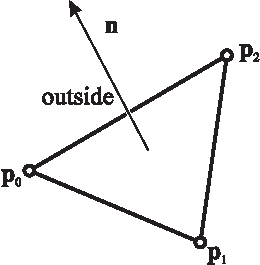
\includegraphics[width=0.25\columnwidth]{figures/triangleNormal}%
\end{center}
\caption{Definition of triangle normals and outside/inside regions in Exudyn: the normal to a triangle with vertex positions $\pv_0$, $\pv_1$, $\pv_2$ is computed from cross product as $\nv = \frac{(\pv_1-\pv_0) \times (\pv_2-\pv_0)}{|(\pv_1-\pv_0) \times (\pv_2-\pv_0)|}$;
the normal $\nv$ then points to the outside region of the mesh or body; the direction of $\nv$ just depends on the ordering of the vertex points (interchange of two points changes the normal direction); correct normals are needed for contact computations as well as for correct shading effects in visualization.}%
\label{fig:triangleNormals}%
\end{figure}
}

%+++++++++++++++++++++++++++++++++++++++++++++++++
%+++++++++++++++++++++++++++++++++++++++++++++++++
\mysubsubsectionlabel{BodyGraphicsData}{sec:bodygraphicsData}
\texttt{BodyGraphicsData} contains a list of \texttt{GraphicsData} items, i.e.\ \texttt{bodyGraphicsData = [graphicsItem1, graphicsItem2, ...]}. Every single \texttt{graphicsItem} may be defined as one of the following structures using a specific 'type'.
The following sections show the different possible types of \texttt{GraphicsData}.

\mysubsubsection{GraphicsData: Line}

GraphicsData \texttt{'type' = 'Line'} draws a polygonal line between all specified points:
\startGenericTable{| p{3cm} | p{2cm} | p{2cm} | p{8.5cm} |}
\rowTableFour{\mybold{Name}}{\mybold{type}}{\mybold{default value}}{\mybold{description}}
\rowTableFour{color}{list}{[0,0,0,1]}{list of 4 floats to define RGB-color and transparency}
\rowTableFour{data}{list}{mandatory}{list of float triples of x,y,z coordinates of the line floats to define RGB-color and transparency}
%\rowTableFour{name}{type}{default}{description}
\finishTable

\noindent \mybold{Example}:
\pythonstyle\begin{lstlisting}
  #rectangle with side length 1:
  graphicsData = {'type':'Line', 
                  'color': [1,0,0,1], #red
                  'data': [0,0,0, 
                           1,0,0, 
                           1,1,0, 
                           0,1,0, 
                           0,0,0]} 

  vGround=VObjectGround(graphicsData=[graphicsData])
  oGround=mbs.AddObject(ObjectGround(referencePosition= [0,0,0], 
                                   visualization=vGround))
\end{lstlisting}
\noindent Certainly this can be done \mybold{much more elegant and shorter with} \texttt{graphics.Lines}:
\pythonstyle\begin{lstlisting}
  import exudyn.graphics as graphics
  graphicsData = graphics.Lines([[0,0,0],[1,0,0],[1,1,0],[0,1,0],[0,0,0]], 
                                color=graphics.color.red)
\end{lstlisting}

\mysubsubsection{GraphicsData: Lines}
%
GraphicsData \texttt{'type': 'Lines'} draws a list of $n$ lines defined by 2 points each:
\startGenericTable{| p{3cm} | p{2cm} | p{2cm} | p{8.5cm} |}
\rowTableFour{\mybold{Name}}{\mybold{type}}{\mybold{default value}}{\mybold{description}}
\rowTableFour{colors}{list}{mandatory}{list [R0,G0,B0,A0, R1,G2,B1,A1, ...] of $2\times n$ x 4 floats to define RGB-color and transparency of line points}
\rowTableFour{points}{list}{mandatory}{list of $2 \times n$ float triples of x,y,z coordinates of the line points; Example for two lines: data=[0,0,0, 1,0,0, 1,0,0, 1,1,0] ... draws a L-shape with side length 1}
\finishTable

\mysubsubsection{GraphicsData: Circle}
%
GraphicsData \texttt{'type' = 'Circle'} draws a polygonal line between all specified points:
\startGenericTable{| p{3cm} | p{2cm} | p{2cm} | p{8.5cm} |}
\rowTableFour{\mybold{Name}}{\mybold{type}}{\mybold{default value}}{\mybold{description}}
\rowTableFour{color}{list}{[0,0,0,1]}{list of 4 floats to define RGB-color and transparency}
\rowTableFour{radius}{float}{mandatory}{radius of circle}
\rowTableFour{position}{list}{mandatory}{list of float triples of x,y,z coordinates of center point of the circle}
\finishTable

\noindent \mybold{Example}:
\pythonstyle\begin{lstlisting}
  graphicsData = {'type':'Circle', 
                  'color': [0,0,1,1],  #blue
                  'radius': 0.5, 
                  'position':[2,3,0]}
\end{lstlisting}

\mysubsubsection{GraphicsData: Text}
%
GraphicsData \texttt{'type' = 'Text'} places the given text at position:
\startGenericTable{| p{3cm} | p{2cm} | p{2cm} | p{8.5cm} |}
\rowTableFour{\mybold{Name}}{\mybold{type}}{\mybold{default value}}{\mybold{description}}
\rowTableFour{color}{list}{[0,0,0,1]}{list of 4 floats to define RGB-color and transparency}
\rowTableFour{text}{string}{mandatory}{text to be displayed, using UTF-8 encoding (see \refSection{sec:utf8})}
\rowTableFour{position}{list}{mandatory}{list of float triples of [x,y,z] coordinates of the left upper position of the text; e.g.\ position=[20,10,0]}
\finishTable

\mysubsubsection{GraphicsData: TriangleList}
%
GraphicsData \texttt{'type' = 'TriangleList'} draws a mesh with flat triangles for given points and connectivity; triangles may look smoothened by using appropriate normals; edges may be added optionally:
\startGenericTable{| p{3cm} | p{2cm} | p{2cm} | p{8.5cm} |}
\rowTableFour{\mybold{Name}}{\mybold{type}}{\mybold{default value}}{\mybold{description}}
\rowTableFour{points}{list}{mandatory}{list [x0,y0,z0, x1,y1,z1, ...] containing $n \times 3$ floats (grouped x0,y0,z0, x1,y1,z1, ...) to define x,y,z coordinates of points, $n$ being the number of points (=vertices)}
\rowTableFour{colors}{list}{[]}{list [R0,G0,B0,A0, R1,G2,B1,A1, ...] containing $n \times 4$ floats to define RGB-color and transparency A of triangle vertices (points), where $n$ must be according to number of points; if field 'colors' does not exist, default colors will be used}
\rowTableFour{normals}{list}{[]}{list [n0x,n0y,n0z, ...] containing $n \times 3$ floats to define normal direction of triangles per point, where $n$ must be according to number of points; if field 'normals' does not exist, default normals [0,0,0] will be used}
\rowTableFour{triangles}{list}{mandatory}{list [T0point0, T0point1, T0point2, ...] containing $n_{trig} \times 3$ integers to define point indices of each vertex of the triangles (=connectivity); point indices start with index 0; the maximum index must be $\le$ points.size()}
\rowTableFour{edges}{list}{[]}{list [L0point0, L0point1, L1point0, L1point1, ...] containing $n_{lines} \times 2$ integers to define point indices of edges drawn on triangle mesh}
\rowTableFour{edgeColor}{list}{[0,0,0,1]}{list of 4 floats to define RGB-color and transparency of edges}
\finishTable
Examples of \texttt{GraphicsData} can be found in the Python examples and in the file \texttt{graphics.py}, see Section \ref{sec:module:graphics}.

%+++++++++++++++++++++++++++++++++++++++++++++++++++++++
%+++++++++++++++++++++++++++++++++++++++++++++++++++++++
\mysubsectionlabel{Character encoding: UTF-8}{sec:utf8}
Character encoding is a major issue in computer systems, as different languages need a huge amount of different characters,
see the amusing blog of Joel Spolsky:\\
\exuUrl{https://www.joelonsoftware.com/2003/10/08/the-absolute-minimum-every-software-developer-absolutely-positively-must-know-about-unicode-and-character-sets-no-excuses/}{The Absolute Minimum Every Software Developer Absolutely, Positively Must Know About Unicode ...}\\
More about encoding can be found in \exuUrl{https://en.wikipedia.org/wiki/UTF-8}{Wikipedia:UTF-8}. UTF-8 encoding tables can be found within the wikipedia article and a comparison with the first 256 characters of unicode is provided at \exuUrl{https://www.utf8-chartable.de/}{UTF-8 char table}.


For short, \codeName\ uses UTF-8 character encoding in texts / strings drawn in OpenGL renderer window.
However, the set of available UTF-8 characters in \codeName\ is restricted to a very small set of characters (as compared to available characters in UTF-8).

\ignoreRST{
The following table shows of available characters (using hex codes, e.g. \texttt{0x20} = \texttt{32}):
\begin{center}
  \footnotesize
  \begin{longtable}{| p{2cm} | p{4cm} | p{8cm} |} 
	\hline
  \bf unicode (hex code) & UTF-8 (hex code) & character \\ \hline
  20 & 20 & ' '\\
  21 & 21 & '!'\\
  $\ldots$ & $\ldots$ & $\ldots$\\
  30 & 30 & '0'\\
  $\ldots$ & $\ldots$ & $\ldots$\\
  39 & 39 & '9'\\
  40 & 40 & '@'\\
  41 & 41 & 'A'\\
  $\ldots$ & $\ldots$ & $\ldots$\\
  5A & 5A & 'Z'\\
  $\ldots$ & $\ldots$ & $\ldots$\\
  7E & 7E & '\textasciitilde{}'\\
  7F & 7F & control, not shown\\
  $\ldots$ & $\ldots$ & $\ldots$\\
  A0 & C2 A0 & no-break space\\
  A1 & C2 A1 & inverted exclamation mark: '!`'\\
  $\ldots$ & $\ldots$ & $\ldots$\\
  BF & C2 BF & inverted '?`'\\
  C0 & C3 80 & A with grave\\
  $\ldots$ & $\ldots$ & $\ldots$\\
  FF & C3 BF & y with diaeresis: '$\ddot{\mathrm{y}}$' \\ \hline
	%++++++++++
	\multicolumn{3}{l}{special characters (selected):} \\ \hline
  %char80:
	 & E2 89 88 & $\approx$ \\
	 & E2 88 82 & $\partial$ \\
	 & E2 88 AB & $\int{}$ \\
	 & E2 88 9A & $\sqrt{}$ \\
	 & CE B1 & $\alpha$ \\
	 & CE B2 & $\beta$ \\
	 & $\ldots$ & (complete list of greek letters see below) \\
   & F0 9F 99 82 & smiley \\
   & F0 9F 98 92 & frowney \\
	 & E2 88 9e & infinity: $\infty$ \\ \hline
  %char90:
	\hline
	%++++++++++
  \end{longtable}
\end{center}
Note, that unicode character codes are shown only for completeness, but they {\bf cannot be encoded in general by \codeName}!
}
Greek characters include: $\alpha, \beta, \gamma, \delta, \varepsilon, \zeta, \eta, \theta, 
\kappa, \lambda, \nu, \xi, \pi, \rho, \sigma, \varphi, \Delta, \Pi, \Sigma, \Omega$.



